\documentclass[12pt]{article}

\usepackage[a4paper,left=2.5cm,right=2.5cm,top=2.5cm,bottom=2.5cm]{geometry}
\usepackage[bahasa]{babel}

\usepackage{lipsum}
\usepackage{graphicx}
\usepackage{hyperref}
\usepackage{tikz}
% \usepackage{biblatex}
% \addbibresource{main.bib}
\usepackage{apacite}
\usepackage{longtable}
% \usepackage[backend=biber,style=apa,citestyle=apa,sorting=ynt]{biblatex}
% \addbibresource{main.bib}
\usepackage{usebib}
\usepackage{enumitem}

\bibinput{main}
\graphicspath{ {./images/} }
% \title{Tugas SPK}
% \author{Ilman Samhabib 91122010\\62/MMSI/SIB}
% \date{\today}

\begin{document}

% \maketitle
% \titlepage
% \newpage
% \tableofcontents
% \newpage
\begin{center}
   \textbf{Tugas: Testing dan Implementasi Sistem}
   \\ Tema: \textbf{Chapter 10 summary}
   \\Ilman Samhabib 9911220\textbf{10} 62/MMSI/SIB

\end{center}


% ====
\subsection*{Definisi \emph{validation testing} }

Pengujian validasi \emph{validation testing} mengevaluasi suatu sistem dalam mode eksekusi untuk memastikan bahwa sistem tersebut berfungsi dengan pada saat beroperasi nantinya.

Tujuan dari uji validitas adalah untuk menilai apakah suatu sistem perangkat lunak berfungsi dengan benar dalam mode eksekusi, meniru lingkungan operasional. Tujuan tersebut adalah memastikan kesiapan perangkat lunak untuk produksi dengan melakukan pengujian yang mengatasi potensi masalah dan penyimpangan dari hasil yang diharapkan. Setiap isu yang teridentifikasi mungkin memerlukan penyesuaian sebelum perangkat lunak diterapkan.


Sedangkan uji verifikasi, yang terjadi pada fase-fase sebelumnya dan memastikan bahwa sistem sesuai dengan spesifikasi. Pengujian verifikasi dilakukan dalam tahap persyaratan, desain, dan program, memastikan bahwa sistem dibangun sesuai dengan spesifikasi.

Sebaliknya,
pengujian validasi,
melibatkan eksekusi perangkat lunak secara keseluruhan untuk mengkonfirmasi fungsinya berjalan dengan baik pada lingkungan yang realistis.

Jika verivikasi pada tahap sebelumnya dilakukan dengan baik, kemunkinan uji validasi yang dilakukan akan lebih sedikit

\subsection*{Kekhawatiran dalam Pengujian Validasi:}
\begin{itemize}
   \item   \textbf{Perangkat Lunak Tidak dalam Mode yang Dapat Diuji:}
         Masalah terkait dengan ketidakmampuan menguji perangkat lunak karena tidak memenuhi kondisi pengujian yang sesuai.
   \item \textbf{Waktu/Sumber Daya yang Tidak Memadai:}
         Keterbatasan waktu atau sumber daya yang dapat mempengaruhi kualitas dan kelengkapan pengujian.
   \item  \textbf{Masalah Signifikan Tidak Terungkap Selama Pengujian:}
         Kekhawatiran bahwa masalah serius mungkin tidak teridentifikasi selama pengujian, yang dapat menyebabkan kesulitan operasional di lingkungan produksi.
\end{itemize}

\subsection*{Membuat Lingkungan Uji:}
\begin{itemize}
   \item Sebuah meja kerja/\emph{test environment / workbench} diilustrasikan untuk menjalankan uji dan kemudian mencatat hasil dari uji teresbut, lingkungan diciptakan  sangat  mirip dengan lingkungan pada fase produksi sistem nantinya.
\end{itemize}
\begin{center}
   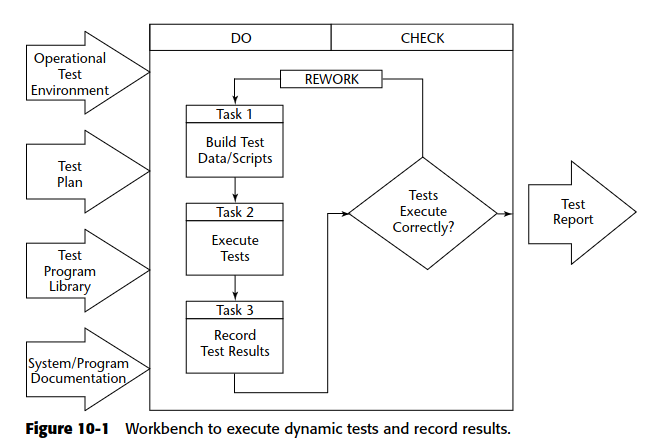
\includegraphics[width=13cm, height=10cm]{images/workbench.png}
\end{center}


\subsection*{Melakukan Pengujian Validasi:}


Setelah disiapkan \emph{workbench} maka ada 3 langkah yang harus dilakukan selanjutnya:
\begin{enumerate}
   \item Membuat \emph{test data}/data input untuk sistem ketika test dijalankan
   \item Mengeksekusi test
   \item Merekam/mendokumentasikan hasil test
\end{enumerate}



% \section*{\emph{Input} Pengujian Validasi:}
% \begin{itemize}
%    \item Masukan untuk pengujian validasi melibatkan rencana uji sistem, data/skrip uji, hasil pengujian verifikasi sebelumnya, dan masukan dari sumber pihak ketiga.
% \end{itemize}

\subsection*{Membangun Data Uji:}
\begin{itemize}
   \item Proses ini melibatkan menciptakan kondisi pemrosesan yang representatif, mempertimbangkan faktor seperti bukti kebenaran, analisis aliran data, dan analisis aliran kontrol.
   \item Berbagai sumber yang dapat dijadikan parameter dalam membuat test data, seperti: dokumentasi sistem, kasus pengguna, generator uji, data produksi, basis data, dan profil operasional.
   \item Penguji harus akrab dengan standar departemen TI untuk merancang file data uji yang memadai, termasuk berbagai data valid dan tidak valid.
   \item Penguji juga harus dapat mengimajinasikan apa output sistem dari setiap input test data yang dirancang tersebut
\end{itemize}

\subsection*{Eksekusi Test}

Persiapan sangat penting untuk menghindari pengujian yang tidak ekonomis dan tidak efektif. Metode yang dapat dijalankan adalah:
\begin{itemize}
   \item \textbf{Pengujian Manual, Regresi, dan Fungsional:}
         \begin{itemize}
            \item Pengujian manual memastikan interaksi pengguna yang benar.
            \item Pengujian regresi memverifikasi dampak instalasi baru pada aplikasi yang sudah ada.
            \item Pengujian fungsional memastikan persyaratan sistem terpenuhi dalam berbagai keadaan.
         \end{itemize}

   \item \textbf{Pengujian Fungsional dan Regresi (Integrasi):}        Memastikan komunikasi yang benar dengan sistem aplikasi terkait.


   \item \textbf{Pengujian Kepatuhan:}
         \begin{itemize}
            \item Termasuk pengujian otorisasi untuk memverifikasi implementasi aturan dengan benar.
            \item Pengujian kinerja, keamanan, integritas file, jejak audit, pengujian kebenaran adalah hal yang penting.
         \end{itemize}

   \item \textbf{Pengujian Pemulihan (Kelangsungan):}  Menguji prosedur alternatif untuk downtime sistem.
         

   \item \textbf{Pengujian Stres (Tingkat Layanan):} Memvalidasi kinerja sistem dalam pemrosesan berkecepatan tinggi.
      

   \item \textbf{Kepatuhan Metodologi:}         
          Pengujian harus mematuhi kebijakan, prosedur, dan dokumentasi yang ditentukan oleh organisasi.
         

   \item \textbf{Pengujian Dukungan Manual (Kemudahan Penggunaan):} Mengevaluasi kegunaan sistem dalam lingkungan yang realistis.
         

   \item \textbf{Inspeksi (Maintainability):}
          Melibatkan inspeksi independen untuk menguji kemampuan pemeliharaan sistem.
         

   \item \textbf{Pengujian Bencana (Portabilitas):}
          Mensimulasikan masalah untuk menguji lingkungan pemrosesan alternatif.
         

   \item \textbf{Pengujian Operasional (Kemudahan Operasi):}
          Dilakukan oleh staf operasional normal untuk menilai keberoperasian sistem tanpa bantuan pengembang.
         
\end{itemize}
Dalam penerapannya ini dilakukan oleh script yang mendefinisikan tiap-tiap \emph{test case} yang sebaiknya mencakupi metode metode diatas, dan dilakukan secara otomatis.



\subsection*{Dokumentasi Hasil Test}
Pendokumentasian hasil uji validasi, dengan merinci atribut kunci untuk setiap kasus uji: 

\begin{enumerate}
   \item Kondisi (apa adanya) .
   \item Kriteria (apa seharusnya). 
   \item Efek (mengapa perbedaan itu signifikan), 
   \item Penyebab (alasan deviasi). 
   
\end{enumerate}
maka Setiap \emph{test case} akan terdokumentasi hal-hal berikut, yang dapat digunakan untuk pemechan masalah:
\begin{itemize}
   
   \item Dokumentasi Deviasi: Deviasi terjadi saat "apa yang ada" tidak sejalan dengan "apa yang seharusnya." Ini melibatkan deskripsi kondisi saat ini (kondisi) dan kriteria yang diinginkan. Deviasi adalah kesenjangan antara kedua keadaan ini.
   
   \item Dokumentasi Efek: Efek menentukan signifikansi dari pernyataan masalah. Ini dinilai berdasarkan efisiensi, ekonomi, dan dampak masa depan yang mungkin. Terukur sedemikian rupa dalam bahasa yang dipahami oleh setiap stakeholder atau manajemen.
   
   \item Dokumentasi Penyebab: Mengidentifikasi penyebab masalah mungkin memerlukan penyelidikan. Penyebab umum termasuk ketidaksesuaian dengan standar, instruksi yang diterbitkan, praktik bisnis yang diterima secara umum, atau praktik yang tidak efisien. Ini dapat dibantu dengan  Pendekatan ilmiah yang melibatkan definisi masalah, analisis alur kerja, identifikasi prosedur, orang yang terlibat, dan pembuatan kembali keadaan.
   
\end{itemize}


% Pernyataan masalah yang baik mencakup semua atribut ini, memastikan kejelasan dan mengatasi pertanyaan potensial.
% \subsection*{Langkah-langkah dalam Pengujian Validasi:}
% \begin{itemize}
%    \item langkah utama: membuat/ \emph{generate} data uji, menjalankan uji, dan mencatat hasil uji.
%    \item Membuat dan menggunakan data uji melibatkan mengidentifikasi sumber daya, kondisi, peringkat, pemilihan kondisi, menentukan hasil yang benar, membuat transaksi uji, mendokumentasikan kondisi, menjalankan uji, dan memverifikasi serta memperbaiki hasil.
% \end{itemize}




% ====
%  \begin{center}
%     Decision Tree(CART)   
%  \end{center}
%   \begin{center}
%     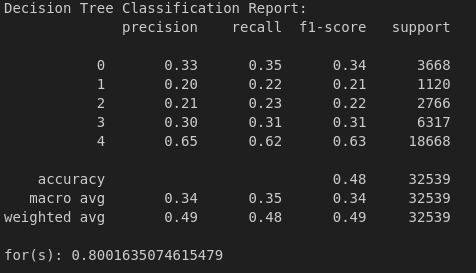
\includegraphics[width=8cm, height=7cm]{images/decision-tree-f1.png}
%     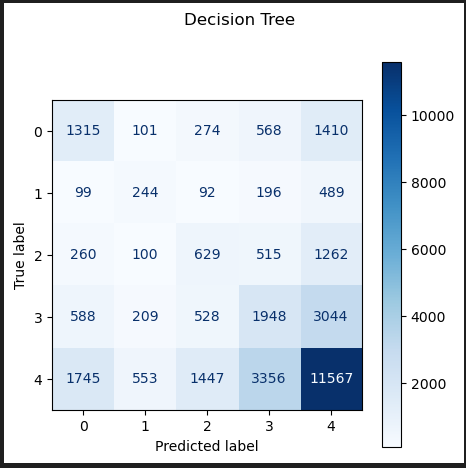
\includegraphics[width=8cm, height=7cm]{images/Dt-confusion.png}   
%  \end{center}
%  \begin{center}
%     KNN(5,uniform)
%  \end{center}
%  \begin{center}
%     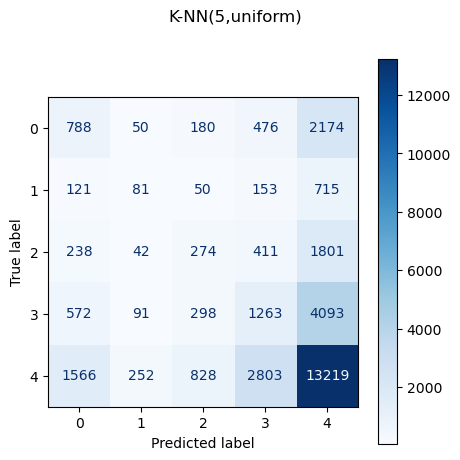
\includegraphics[width=8cm, height=7cm]{images/knn-f1.png}
%     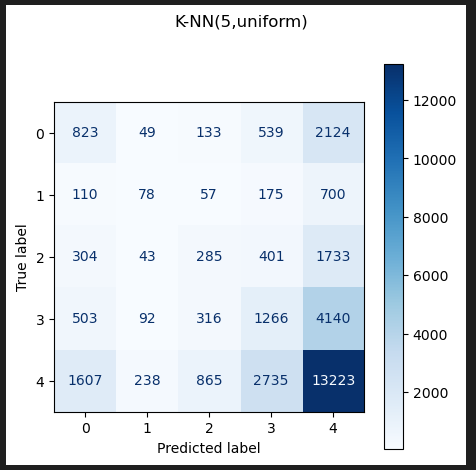
\includegraphics[width=8cm, height=7cm]{images/knn-confusion.png}
%  \end{center}
%  \begin{center}
%     Random Forest
%  \end{center}
%  \begin{center}
%     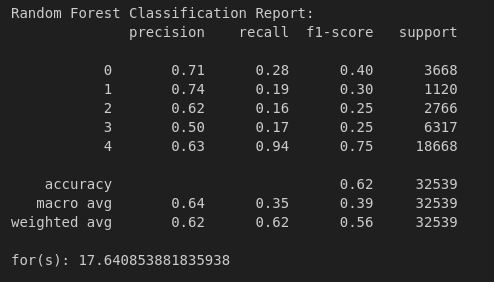
\includegraphics[width=8cm, height=6cm]{images/random-forest-f1.png}
%     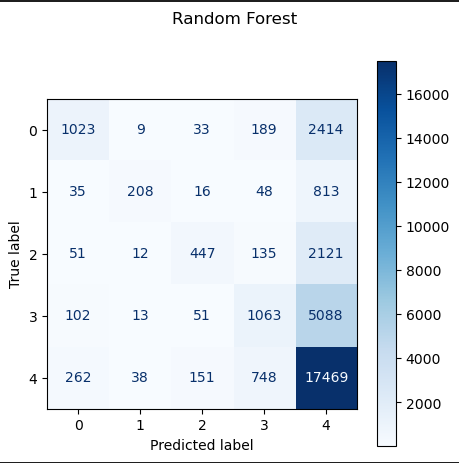
\includegraphics[width=8cm, height=6cm]{images/rf-confusion.png}
%  \end{center}
%  \begin{center}
%     XGBoost
%  \end{center}




% \bibliographystyle{apacite}
% \bibliography{main}
% \printbibliography


\end{document}